\documentclass[12pt,oneside,letterpaper]{article}

\usepackage[canadien]{babel}
\usepackage[utf8]{inputenc}
\usepackage[T1]{fontenc}
\usepackage{lmodern}
\usepackage{graphicx}
\usepackage[letterpaper]{geometry}
\usepackage[americanvoltages,americancurrents, siunitx]{circuitikz}
\usetikzlibrary{babel}
\usepackage{caption}
\usepackage{subfig}
\usepackage{amsmath}
\usepackage{hyperref}
\usepackage[all]{hypcap}


\captionsetup{font=small,labelfont=bf,margin=0.1\textwidth}
\pagestyle{myheadings}
\markboth{GPH-2006/PHY-2002~---~Composants~non~linéaires}{GPH-2006/PHY-2002~---~Composants~non~linéaires}


\begin{document}


\title{\textbf{Complément}\\Composants non linéaires}
\author{Jean-Raphaël Carrier \& Claudine Allen}
\date{}
\maketitle


\section{Diode}

Une diode est un composant électronique non linéaire et polarisé. La polarisation implique que le comportement d'une diode dépend du sens du branchement. La plupart des multimètres ont une fonction \textit{diode check} qui permet de s'assurer que le branchement est adéquat.

\begin{center}
\begin{circuitikz} \draw
(0,0) to[D] (2,0)
{[anchor=south east] (0,0) node{Anode (+)}}
{[anchor=south west] (2,0) node{Cathode (--)}}
;\end{circuitikz}
\end{center}

La diode agit comme un clapet dans un circuit :  elle permet au courant électrique de circuler dans un sens, mais pas dans l'autre. Dans une diode, le courant circule de l'anode (borne positive) vers la cathode (borne négative). Pour faire circuler un courant dans le sens normal (polarité directe), une diode nécessite une tension minimale $v_d$. Cette tension $V_d$ aux bornes de la diode demeurera environ constante\footnote{Les diodes usuelles ont une tension $v_d$ de l'ordre de quelques dixièmes de volt.}, même si le courant qui la traverse augmente. Autrement dit, la chute de potentiel est indépendante du courant. Lorsque la diode est employée en sens inverse, aucun courant ne la traverse, indépendamment de la tension appliquée à ses bornes.

Pour une diode idéale, la relation non linéaire entre le courant et la tension est donc une droite horizontale qui devient une droite verticale à $v_d$, ce qui est illustré à la figure~\ref{diode-ideale}. Mathématiquement, cette relation peut s'exprimer ainsi:
\begin{flalign*}
&&&&i\!\left(t\right)=0 &\;& -\infty<v\!\left(t\right)\le v_d&&&&\\
&&&&v\!\left(t\right)=v_d &\;& 0<i\!\left(t\right)<\infty&&&&
\end{flalign*}
\begin{figure}[h]
\begin{center}
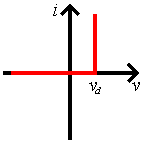
\includegraphics[width=0.4\textwidth]{diode-ideale}
\caption{\label{diode-ideale}Courbe $i$--$v$ idéalisée d'une diode.}
\end{center}
\end{figure}

Comme la résistance est seulement une constante de proportionnalité entre la tension et le courant, il est habituel de définir une version instantanée de la résistance dans le cas des diodes, soit:
\begin{equation*}
R_D\!\left(t\right)=\frac{\textrm{d}v\!\left(t\right)}{\textrm{d}i\!\left(t\right)}.
\end{equation*}
Cette résistance exprime l'opposition au passage du courant de la diode pour une tension donnée et sa valeur n'est pas constante, on la nomme donc \textit{résistance dynamique}. Dans le cas de la diode idéale, on voit que $R_D \rightarrow \infty$ pour $v\!\left(t\right) < v_d$ et $R_D=0$ pour $v\!\left(t\right) > v_d$.

Contrairement aux résistance, bobine et condensateur, une diode n'a pas de paramètre unique qui caractérise sa relation entre la tension et le courant. Toutefois, ceci ne veut pas dire que toutes les diodes sont pareilles. En fait, les diodes standards sont caractérisées par quelques critères, dont : la tension inverse de pointe et le courant maximal.

La tension inverse de pointe est la tension qui doit être appliquée pour qu'un courant commence à traverser la diode dans le sens inverse. En d'autres mots, elle équivaut à la tension nécessaire pour \textit{briser} la diode.

Le courant maximal équivaut à la valeur du plus grand courant qui peut traverser une diode en polarité directe sans que celle-ci ne soit endommagée. Si un courant supérieur est fourni, la diode va chauffer et son comportement risque de ne plus être celui souhaité.


\subsection{Diode Zener}

Les diodes Zener sont conçues pour laisser passer plus facilement le courant en polarisation inverse sans briser. La tension inverse de pointe est donc beaucoup plus faible pour les diodes Zener que pour les autres diodes. On parle alors de \textit{tension Zener}. Le schéma d'une diode Zener est sensiblement différent d'une diode standard.

\begin{center}
\begin{circuitikz} \draw
(0,0) to[zD] (2,0)
;\end{circuitikz}
\end{center}

La valeur de la tension Zener à partir du moment qu'un courant inverse circule varie très peu avec le courant. Placée en parallèle avec un autre élément, elle peut être utilisée pour limiter la tension aux bornes de ce composant et ainsi le protège des possibles fluctuations du circuit. Pour ce faire, autant de courant que nécessaire circule dans la diode Zener afin de garder la tension constante dans les deux branches du circuit (puisque deux composants en parallèle ont la même tension).

Même si ces diodes sont conçues pour laisser passer le courant inverse, elles peuvent tout de même être endommagées si la puissance dissipée excède un certain seuil.


\subsection{Diode électroluminescente et photodiode}

Certaines diodes émettent de la lumière visible ou infrarouge en polarité directe : on parle alors de diodes électroluminescentes, souvent abrégées DEL ou LED (de l'anglais \textit{light-emitting diode}). La puissance lumineuse émise est directement proportionnelle au courant qui traverse la LED après qu'un seuil de courant minimum soit dépassé.

À l'inverse, une diode peut absorber de la lumière pour générer du courant. Les diodes qui sont optimisées pour cette fonction sont nommées photodiodes. La relation entre courant et puissance lumineuse est linéaire sur une plage d'opération normale de la photodiode, mais la constante de proportionnalité sera dépendante de la longueur d'onde.

\begin{center}
\begin{circuitikz} \draw
(0,0) to[leD] (2,0)
(5,0) to[pD] (7,0)
(1,-0.5) node[below]{Diode électroluminescente}
(6,-0.5) node[below]{Photodiode}
;\end{circuitikz}
\end{center}


\section{Transistor}

Les transistors sont des tripôles (donc des \textit{triodes}), c'est-à-dire qu'ils possèdent trois connexions : la troisième connexion contrôle le comportement du dipôle formé par les deux autres. Il existe différents types de transistors, les plus répandus se répartissant en deux catégories, soient les transistors bipolaires, ou BJT (de l'anglais \textit{bipolar junction transistor}) et les transistors à effet de champ, ou FET (\textit{field-effect transistors}). Les connexions d'un transistor bipolaire sont : l'émetteur, le collecteur et la base qui est la connexion de contrôle. Dans le cas des transistors à effet de champ, ces mêmes connexions s'appellent respectivement : le drain, la source et la grille. Les transistors BJT sont des dispositifs contrôlés par le courant circulant dans la base, alors que les transistors FET le sont par la différence de potentiel entre la grille et la source.

\begin{center}
\begin{circuitikz} \draw
(0,0) node[npn](npn){}
(npn.base) node[anchor=east] {B}
(npn.collector) node[anchor=south] {C}
(npn.emitter) node[anchor=north] {E}
(4,0) node[pjfet](pjfet){}
(pjfet.G) node[anchor=east] {G}
(pjfet.S) node[anchor=south] {S}
(pjfet.D) node[anchor=north] {D}
;\end{circuitikz}
\end{center}

Grossièrement, les transistors peuvent être utilisés de deux façons dans un circuit : comme interrupteur ou encore comme amplificateur. Dans un transistor BJT\footnote{Seuls les transistors bipolaires (BJT) seront vus dans ce cours.}, le courant circule du collecteur vers l'émetteur et la valeur de ce courant est contrôlée par la base.

Lorsque le courant circulant dans la base est inférieur à une certaine valeur seuil, le transistor agit comme un interrupteur ouvert : aucun courant ne circule entre le collecteur et l'émetteur. À l'inverse, lorsqu'un grand courant circule dans la base, le courant collecteur--émetteur est maximal : le transistor agit alors comme un interrupteur fermé. Entre ces deux régimes, le courant entre le collecteur et l'émetteur sera proportionnel au courant circulant dans la base. Dans ce dernier cas, le transistor agit comme un amplificateur.


\end{document}

Écrit par Jean-Raphaël Carrier
Dernière modification : 11 janvier 2014
